\SourcePage{417}{420}
\section{Predissociation}

The theory of diatomic molecules developed in this chapter rests chiefly on the assumption that the molecular wave function separates into a product of an electronic wave function (depending parametrically on the internuclear distance) and a wave function for the nuclear motion. This assumption amounts to neglecting certain small terms in the exact molecular Hamiltonian that describe the coupling of nuclear motion to the electrons.

When these terms are included as perturbations, transitions arise between different electronic states. Of particular physical importance are transitions for which at least one state belongs to the continuous spectrum.

Figure~30 shows the potential-energy curves of two electronic terms (more precisely, the effective potential energy $U_J$ in specified rotational states of the molecule). The energy $E'$ is that of a particular vibrational level of a stable molecule in electronic state 2. In state 1 this energy lies in the continuous spectrum. Thus a transition from state 2 to state 1 causes spontaneous breakup of the molecule; this phenomenon is called \emph{predissociation}.\footnote{Curve 1 need not have a minimum at all if it corresponds to purely repulsive forces between the atoms.} As a result of predissociation, the discrete-spectrum state represented by curve 2 actually has a finite lifetime. This means that the discrete

\begin{figure}[ht]
\centering
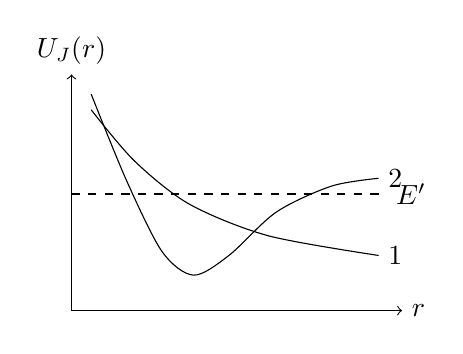
\begin{tikzpicture}[x=1cm,y=1cm]
\draw[->] (0,0)--(4.2,0) node[right]{$r$}; \draw[->] (0,0)--(0,3) node[above]{$U_J(r)$};
\draw[smooth] plot coordinates {(.25,2.55)(.8,1.9)(1.5,1.35)(2.5,.95)(3.9,.7)} node[right]{1};
\draw[smooth] plot coordinates {(.25,2.75)(.7,1.65)(1.15,.75)(1.55,.45)(2,.7)(2.6,1.25)(3.3,1.58)(3.9,1.68)} node[right]{2};
\draw[dashed] (0,1.48)--(4,1.48) node[right]{$E'$};
\end{tikzpicture}
\caption*{Fig. 30}
\end{figure}

\SourcePage{418}{421}
energy level is broadened: it acquires a certain width (see the end of \S~44).

If instead the total energy $E$ lies above the dissociation limit in both states, a transition from one state to the other corresponds to a so-called \emph{collision of the second kind}. A transition $1\to2$, for example, means that two colliding atoms pass into excited states and separate with reduced kinetic energy (as $r\to\infty$, curve 1 lies below curve 2; the difference $U_2(\infty)-U_1(\infty)$ is the atomic excitation energy).

Because of the large nuclear mass, the nuclear motion is semiclassical. The problem of finding the probability of these transitions therefore belongs to the class discussed in \S~52. The general considerations given there show that the transition probability is governed by the point at which the transition could occur classically.\footnote{Or the point $r=0$, at which the potential energy becomes infinite.} Since the total energy of the two-atom system (the molecule) is conserved in the transition, its ``classical possibility'' requires equality of the effective potential energies: $U_{J1}(r)=U_{J2}(r)$. The total molecular angular momentum is also conserved, so the centrifugal energies are the same in the two states. The condition therefore reduces to equality of the potential energies,
\begin{equation}U_1(r)=U_2(r),\tag{90.1}\end{equation}
and contains no angular momentum at all.

If (90.1) has no real root in the classically accessible region (where $E>U_{J1},U_{J2}$), then by \S~52 the transition probability is exponentially small.\footnote{A peculiar situation occurs for a transition involving a molecular term that may be formed from two different pairs of atomic states (see the end of \S~85), so that toward increasing distances the potential-energy curve seems to divide into two branches. The transition probability is then appreciably enhanced; for an example see A.~I.~Voronin and E.~E.~Nikitin, \emph{Optics and Spectroscopy} \textbf{25}, 803 (1968).} Transitions have appreciable probability only if the potential-energy curves cross within the classically accessible region (as in Fig.~30). In that event the exponent in (52.1) vanishes (so that formula is, of course, inapplicable), and the transition probability is determined by a nonexponential expression, derived below. Condition (90.1) may

\SourcePage{419}{422}
also be interpreted directly as follows. Equal potential (and total) energies imply equal momenta. Thus (90.1) may be written
\begin{equation}r_1=r_2,\qquad p_1=p_2,\tag{90.2}\end{equation}
where $p$ is the momentum of the relative radial motion of the nuclei, and the indices 1 and 2 refer to the two electronic states. Hence at the instant of transition the internuclear distance and nuclear momentum may be said to remain unchanged (the so-called \emph{Franck--Condon principle}). Physically, this is because electronic velocities are large compared with nuclear velocities, so ``during the electronic transition'' the nuclei have no time to change their positions or velocities appreciably.

The selection rules for these transitions are easily established. First, there are two evident exact rules: the total angular momentum $J$ and the sign (positive or negative; see \S~86) of the term must not change. This follows directly because conservation of total angular momentum and invariance of the wave-function character under inversion of the coordinate system are exact laws for every closed system of particles.

There is also, to high accuracy, a rule forbidding transitions between states of different parity in a molecule of identical atoms. Indeed, the parity of the state is uniquely fixed by the nuclear spin and the sign of the term. The sign is conserved exactly, while the nuclear spin is conserved to high accuracy because of its weak interaction with the electrons.

The requirement that the potential-energy curves have a crossing point means that the terms must have different symmetries (see \S~79). Consider transitions that arise already in first-order perturbation theory. We first note that the Hamiltonian terms producing these transitions are precisely those responsible for the $\Lambda$-doubling of the levels. They include, in the first place, terms describing the spin--orbit interaction. These are products of two axial vectors, one spin-like and the other coordinate-like; it should be stressed, however, that these vectors are by no means simply $\widehat{\mathbf S}$ and $\widehat{\mathbf L}$. They therefore have nonzero matrix elements for transitions in which $S$ and $\Lambda$ change by $0,\pm1$.

\SourcePage{420}{423}
The case $\Delta S=\Delta\Lambda=0$ with $\Lambda\ne0$ must be excluded, since the symmetry of the term would then not change at all in the transition. A transition between two $\Sigma$ terms is possible if one is a $\Sigma^+$ term and the other a $\Sigma^-$ term (an axial vector has matrix elements only for transitions between $\Sigma^+$ and $\Sigma^-$; see \S~87).

The Hamiltonian term describing the coupling between molecular rotation and orbital angular momentum is proportional to $\widehat{\mathbf J}\widehat{\mathbf L}$. Its matrix elements are nonzero for transitions with $\Delta\Lambda=\pm1$ and no change in spin (matrix elements with $\Delta\Lambda=0$ are possessed only by the $\zeta$ component of the vector, namely $L_\zeta$, but $L_\zeta$ is diagonal in the electronic states).

Besides these terms there is a perturbation due to the nuclear kinetic-energy operator acting not only on the nuclear wave function but also on the electronic function, which depends parametrically on $r$. The corresponding Hamiltonian terms have the same symmetry as the unperturbed Hamiltonian. They can therefore produce transitions only between electronic terms of the same symmetry, whose probability is negligible because such terms do not cross.

We now calculate the transition probability explicitly. For definiteness, consider a collision of the second kind. By the general formula (43.1), the required probability is
\begin{equation}w=\frac{4\pi^2}{\hbar^2}\left|\int\chi_{\text{nuc},2}V(r)\chi_{\text{nuc},1}\,dr\right|^2,\tag{90.3}\end{equation}
where $\chi_{\text{nuc}}=r\psi_{\text{nuc}}$, and $V(r)$ is the perturbing energy. The final wave function $\chi_{\text{nuc},2}$ must be normalized to an energy delta function. With this normalization, the semiclassical function is
\begin{equation}\chi_{\text{nuc},2}=\sqrt{\frac2{\pi\hbar v_2}}\cos\left(\frac1\hbar\int_{a_2}^r p_2\,dr-\frac\pi4\right).\tag{90.4}\end{equation}
The initial-state wave function is written

\SourcePage{421}{424}
\begin{equation}\chi_{\text{nuc},1}=\frac2{\sqrt{v_1}}\cos\left(\frac1\hbar\int_{a_1}^r p_1\,dr-\frac\pi4\right).\tag{90.5}\end{equation}
It is normalized so that the current density in each of the two traveling waves is unity. Substitution of these functions in (90.3) gives the dimensionless transition probability $w$, which may be regarded as the probability for two passages of the nuclei through $r=r_0$.

The matrix element contains a product of cosines, which we expand into cosines of the sum and difference of their arguments. Near $r=r_0$ only the latter cosine is relevant, so that
\[
w=\frac4{\hbar^2}\left|\int\frac{V(r)}{\sqrt{v_1v_2}}\cos\left(\frac1\hbar\int_{a_1}^r p_1dr-\frac1\hbar\int_{a_2}^r p_2dr\right)dr\right|^2.
\]
The integral converges rapidly away from the crossing point. Expanding the argument in powers of $\xi=r-r_0$ and recalling that $p_1=p_2$ at the crossing, we find
\[
\int^r p_1dr-\int^r p_2dr\approx S_0+\frac12\left(\frac{dp_1}{dr}-\frac{dp_2}{dr}\right)_0\xi^2.
\]
Differentiating $p_1^2/2\mu+U_1=p_2^2/2\mu+U_2$ gives
\[
v_1\frac{dp_1}{dr}-v_2\frac{dp_2}{dr}=F_1-F_2,
\]

\SourcePage{422}{425}
and hence
\[
\int^r p_1dr-\int^r p_2dr\approx S_0+\frac{F_1-F_2}{2v}\xi^2.
\]
Using the familiar integral, we finally obtain
\begin{equation}w=\frac{8\pi V^2}{\hbar v|F_2-F_1|}\cos^2\left(\frac{S_0}{\hbar}+\frac\pi4\right).\tag{90.6}\end{equation}
The quantity $S_0/\hbar$ is large and changes rapidly with the energy. On averaging, the squared cosine is replaced by its mean value, and
\begin{equation}w=\frac{4\pi V^2}{\hbar v|F_2-F_1|}.\tag{90.7}\end{equation}
(L.~D.~Landau, 1932). All quantities on the right are evaluated at the crossing point.

For predissociation, the decay probability per unit time is obtained by multiplying $w$ by $\omega/2\pi$:
\begin{equation}\frac1\tau=\frac{2\omega V^2}{\hbar v|F_2-F_1|}.\tag{90.8}\end{equation}

In speaking of crossing terms, we meant eigenvalues of the unperturbed Hamiltonian $\widehat H_0$, without the terms $\widehat V$ that produce transitions. When these terms are included, the crossing disappears and the curves separate as in Fig.~31.

\SourcePage{423}{426}
Let $U_{J1}(r)$ and $U_{J2}(r)$ be two eigenvalues of $\widehat H_0$. The method of \S~79 gives
\begin{equation}U_{b,a}(r)=\frac12(U_{J1}+U_{J2})\pm\frac12\sqrt{(U_{J1}-U_{J2})^2+4V^2}.\tag{90.9}\end{equation}
The level separation is
\begin{equation}\Delta U=\sqrt{(U_{J1}-U_{J2})^2+4V^2},\tag{90.10}\end{equation}
and its minimum at $r=r_0$ is
\begin{equation}(\Delta U)_{\min}=2|V(r_0)|.\tag{90.11}\end{equation}
Near this point,
\begin{equation}\Delta U=\sqrt{(F_2-F_1)^2(r-r_0)^2+4V^2}.\tag{90.12}\end{equation}

\begin{figure}[ht]
\centering
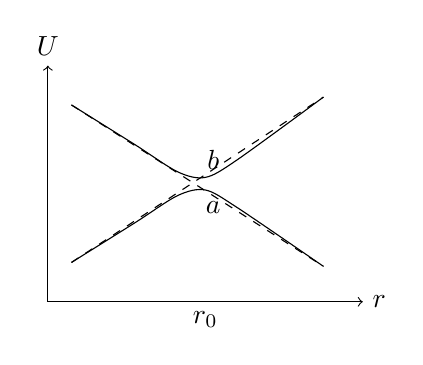
\begin{tikzpicture}[x=1cm,y=1cm]
\draw[->] (0,0)--(4,0) node[right]{$r$}; \draw[->] (0,0)--(0,3) node[above]{$U$};
\draw[dashed] (.3,.5)--(3.5,2.6); \draw[dashed] (.3,2.5)--(3.5,.45);
\draw[smooth] plot coordinates {(.3,2.5)(1.1,2)(1.65,1.65)(2,1.58)(2.4,1.8)(3.5,2.6)};
\draw[smooth] plot coordinates {(.3,.5)(1.1,1)(1.65,1.35)(2,1.42)(2.4,1.2)(3.5,.45)};
\node at (2.1,1.8){$b$}; \node at (2.1,1.2){$a$}; \node[below] at (2,0){$r_0$};
\end{tikzpicture}
\caption*{Fig. 31}
\end{figure}

These formulas require $(\Delta U)_{\min}$ to be small compared with the distance to the other terms. If condition (90.19) is not satisfied, ordinary perturbation theory for the transition probability is inapplicable and a more general treatment is required.

\SourcePage{424}{427}
In the neighborhood of the crossing, treating the nuclear motion semiclassically, we replace the velocity operator by the constant $v$ and put $\xi=r-r_0=vt$. The problem reduces to the equation
\begin{equation}i\hbar\frac{\partial\Psi}{\partial t}=[\widehat H_0(t)+\widehat V(t)]\Psi.\tag{90.13}\end{equation}
Let $\psi_a,\psi_b$ be the electronic states of curves $a,b$. We seek the solution as
\begin{equation}\Psi=a(t)\psi_a+b(t)\psi_b.\tag{90.14}\end{equation}
With the boundary condition $a=1,b=0$ as $t\to-\infty$, the quantity $|b(\infty)|^2$ is the probability of a transition from curve $a$ to curve $b$ in one passage through the point. For two passages the transition proceeds by the paths $a\to b\to b$ or $a\to a\to b$, so
\begin{equation}w=2|b(\infty)|^2[1-|b(\infty)|^2].\tag{90.15}\end{equation}

The value of $b(\infty)$ can be found by the method of \S~53.\footnote{In \S~53 the process was assumed adiabatic throughout. Here adiabaticity may fail in the immediate vicinity of $r_0$, but only adiabaticity at large $|t|$ and the possibility of restricting the treatment to two levels are essential.}

\SourcePage{425}{428}
The curves $U_a(t)$ and $U_b(t)$ cross at the imaginary points
\begin{equation}t_0^{(\pm)}=\pm i\frac{2V}{|F_2-F_1|v}=\pm i\tau_0.\tag{90.16}\end{equation}
Passing into the complex $t$ plane and going around the point $t_0^{(+)}$, with
\begin{equation}\Delta U=\sqrt{(F_2-F_1)^2v^2t^2+4V^2},\tag{90.17}\end{equation}
we finally obtain
\begin{equation}w=2\exp\left(-\frac{2\pi V^2}{\hbar v|F_2-F_1|}\right)\left[1-\exp\left(-\frac{2\pi V^2}{\hbar v|F_2-F_1|}\right)\right].\tag{90.18}\end{equation}
(C.~Zener, 1932). The probability is small in both limiting cases. For $V^2\gg\hbar v|F_2-F_1|$ it is

\SourcePage{426}{429}
exponentially small (the adiabatic case), while for
\begin{equation}V^2\ll\hbar v|F_2-F_1|\tag{90.19}\end{equation}
formula (90.18) reduces to (90.7). Equation (90.17) shows that $\tau\sim|V|/(|F_2-F_1|v)$ is the ``time taken by the nuclei to pass'' the crossing point.

We conclude with a phenomenon related to predissociation, the so-called perturbations in the spectrum of diatomic molecules. If two discrete molecular levels $E_1,E_2$ are close, the possibility of a transition shifts them. By (79.4),
\begin{equation}E=\frac{E_1+E_2}{2}\pm\sqrt{\left(\frac{E_1-E_2}{2}\right)^2+|V_{12}^{\text{nuc}}|^2}.\tag{90.20}\end{equation}
The two levels move apart, and their separation increases as $|E_1-E_2|$ decreases. The matrix element $V_{12}^{\text{nuc}}$ is calculated as above, except that the discrete-spectrum nuclear functions are normalized to unity. Comparison gives
\begin{equation}|V_{12}^{\text{nuc}}|^2=w\frac{\hbar\omega_1}{2\pi}\frac{\hbar\omega_2}{2\pi}.\tag{90.21}\end{equation}

\SourcePage{427}{430}
\ProblemHeading[1] Determine the total cross section for collisions of the second kind as a function of the kinetic energy $E$ of the colliding atoms, for transitions due to the spin--orbit interaction (L.~D.~Landau, 1932).

\SolutionHeading Since the nuclear motion is semiclassical, we may introduce the impact parameter $\rho$ and write $d\sigma=2\pi\rho\,d\rho\,w(\rho)$. For the spin--orbit interaction the matrix element $V(r)$ is independent of angular momentum. The velocity at the crossing point is
\[
v=\sqrt{\frac2\mu\left(E-U-\frac{\rho^2E}{r_0^2}\right)}.
\]
Integration over $\rho$ gives
\[
\sigma=\frac{4\sqrt{2\mu}\pi^2V^2r_0^2}{\hbar|F_2-F_1|}\frac{\sqrt{E-U}}{E}.
\]

\ProblemHeading[2] The same for transitions due to the coupling of molecular rotation to orbital angular momentum (L.~D.~Landau, 1932).

\SolutionHeading The matrix element has the form $V(r)=MD/\mu r^2$, where $D(r)$ is a matrix element of the electronic orbital angular momentum. In the same way we obtain
\[
\sigma=\frac{16\sqrt2\pi^2D^2(E-U)^{3/2}}{3\hbar\mu r_0^2|F_2-F_1|E}.
\]

\ProblemHeading[3] Determine the transition probability for energies $E$ close to the value $U$ of the potential energy at the crossing point.

\SolutionHeading For small $E-U$, formula (90.7) is inapplicable. Near the crossing we replace the curves by the straight lines $U_1=U-F_1\xi$, $U_2=U-F_2\xi$, $\xi=r-r_0$. The wave functions coincide with those for one-dimensional motion in a uniform field. Calculation in the momentum representation gives

\SourcePage{428}{431}
\begin{equation}
w=\frac{4\pi V^2(2\mu)^{2/3}}{\hbar^{4/3}(F_1F_2)^{1/2}(F_2-F_1)^{2/3}}
\Phi^2\!\left[-\frac{E-U}{\hbar^{2/3}}\left(\frac{2\mu(F_2-F_1)^2}{F_1^2F_2^2}\right)^{1/3}\right],
\tag{90.22}
\end{equation}
where $\Phi$ is the Airy function (see \S~b of the Mathematical Appendices). For large $E-U$, this formula reduces to (90.7).

\ProblemHeading[4] Determine the charge-transfer probability in a distant slow ($v\ll1$) collision between a hydrogen atom and a proton (O.~V.~Firsov, 1951).\footnote{Atomic units are used in this problem.}

\SolutionHeading Regard the system $\mathrm H+\mathrm H^+$ as a hydrogen molecular ion (see the problem in \S~81). Charge transfer consists in the electron passing from the state $\psi_1$, localized at the first nucleus, to the state $\psi_2$ near the second. The stationary states are
\[
\psi_{g,u}=\frac1{\sqrt2}(\psi_1\pm\psi_2).
\]
Their energies are $U_{g,u}(R)$. For a prescribed slow classical motion of the nuclei, the time dependence is specified by the factors $\exp[-i\int U_{g,u}(t)dt]$. As $t\to\infty$, the charge-transfer probability is
\[
w=\sin^2\eta,\qquad \eta=\frac12\int_{-\infty}^{\infty}(U_u-U_g)dt.
\]
For large impact parameters $\rho$, put $R=\sqrt{\rho^2+v^2t^2}$ and use formula (4) from the problem in \S~81:
\[
\eta=\frac4v\int_\rho^\infty\frac{R^2e^{-R-1}}{\sqrt{R^2-\rho^2}}\,dR.
\]
For $\rho\gg1$, putting $R=\rho(1+x)$, we obtain
\[
\eta=\frac{2\sqrt{2\pi}}{ev}\rho^{3/2}e^{-\rho}.
\]
